

\documentclass[conference]{IEEEtran}
\usepackage{graphicx}



\ifCLASSINFOpdf
\else
\fi
\hyphenation{op-tical net-works semi-conduc-tor}


\begin{document}

\title{A study of RISC, CISC to ARM architecture, and System on Chip }


% author names and affiliations
% use a multiple column layout for up to three different
% affiliations
\author{\IEEEauthorblockN{Chihsiang Wang}
\IEEEauthorblockA{Computer Science\\
University of Idaho\\
Email: wang0162@vandals.uidaho.edu}}

% conference papers do not typically use \thanks and this command
% is locked out in conference mode. If really needed, such as for
% the acknowledgment of grants, issue a \IEEEoverridecommandlockouts
% after \documentclass

% for over three affiliations, or if they all won't fit within the width
% of the page, use this alternative format:
% 
%\author{\IEEEauthorblockN{okok\IEEEauthorrefmark{1}}

%\IEEEauthorblockA{\IEEEauthorrefmark{1}School of Electrical and Computer Engineering\\
%Georgia Institute of Technology,
%Atlanta, Georgia 30332--0250\\ Email: see http://www.michaelshell.org/contact.html}
%\IEEEauthorblockA{\IEEEauthorrefmark{2}Twentieth Century Fox, Springfield, USA\\
%Email: homer@thesimpsons.com}
%\IEEEauthorblockA{\IEEEauthorrefmark{3}Starfleet Academy, San Francisco, California 96678-2391\\
%Telephone: (800) 555--1212, Fax: (888) 555--1212}
%\IEEEauthorblockA{\IEEEauthorrefmark{4}Tyrell Inc., 123 Replicant Street, Los Angeles, California 90210--4321}}




% use for special paper notices
%\IEEEspecialpapernotice{(Invited Paper)}




% make the title area
\maketitle

% As a general rule, do not put math, special symbols or citations
% in the abstract
\begin{abstract}
ARM architecture is widely used in the contemporary embedded system devices, Smart Phones, Tablets or other personal devices. These devices  are expected to be smaller and faster for users, System on Chip(SoC) are designing to and this is becoming an appreciable market. To react to the rapid demand in the market, traditional hardware component has been evolved  to be a smaller and faster personal devices. Multiprocessor System on Chip (MPSoCs) has been noticed and studied at the recent researches, and it's also becoming a mainstream hardware component to meet market demands. This paper surveys the research of the advantage of Reduced Instruction Set Computing(RISC), and the benefits with microprocessors. Also this paper discuses the ARM architecture and the SoCs history and its adventages.
\end{abstract}

\begin{IEEEkeywords}
ARM Architecture, MultiProcessor, RISC, SoCs.
\end{IEEEkeywords}
% no keywords




% For peer review papers, you can put extra information on the cover
% page as needed:
% \ifCLASSOPTIONpeerreview
% \begin{center} \bfseries EDICS Category: 3-BBND \end{center}
% \fi
%
% For peerreview papers, this IEEEtran command inserts a page break and
% creates the second title. It will be ignored for other modes.
\IEEEpeerreviewmaketitle



\section{Introduction}
Embedded System Devices are prevailing in several areas. Personal smart phone, tablet and many other mobile devices are becoming increasingly important. This paper focus on processors architecture, include Reduced Instruction Set Computing(RISC), ARM architecture, System on Chip(SoC) and Multiprocessors.
\section{Reduced Instruction Set Computing}
\subsection{What is RISC}
RISC (Reduced Instruction Set Computing) is a strategy of a processor design which simplified instruction set, so that it can operate at a higher speed (execute more instructions per second) and higher performance(fewer processor cycles per instructions). The general concept of RISC is that a system uses smaller and highly optimized instruction sets, instead of complex instruction sets. Another common characteristic of RISC system is that it uses the Load / Store Architecture - memory is normally accessed only through specific instructions, rather than accessed as part of other instructions like ADD.\cite{A} The opposite architecture is called Complex Instruction Set Computing(CISC). A brief comparison table between the RISC and CISC is shown in \textit{\textbf{Table 1}}.\\

\begin{table}[h]
\centering
\caption{CISC \& RISC}
\label{my-label}
\begin{tabular}{ll}
\hline
CISC                                              & RISC                                      \\ \hline
Emphasis on Hardware                              & Emphasis on Software                      \\
Multiple Ins. Sizes and Formats            & Ins. of Same Set with Few Formats \\
Less Registers                                    & Uses More Registers                       \\
More Addressing Modes                             & Fewer Addressing Modes                    \\
Extensive Use of Microprogramming                 & Complexity in Computer                    \\
Ins. takes a Varying Amount of Cycle Time & Ins. take one Cycle Time          \\
Pipelining is Difficult                           & Pipelining is Easy                        \\ \hline
\end{tabular}
\end{table}

\subsection{History and Feature of RISC}
The first RISC projects came from IBM, Stanford and UC-Berkeley in the late 70s and early 80s. The IBM 801, Stanford MIPS, and Berkeley RISC 1 and 2 were all designed with a similar philosophy which has become known as RISC. Before RISC philosophy became prominent, most of systems architecture were tried to design the instruction sets which can directly support high level programming\cite{C}. In the other words, scientist tried to construct various procedures into a single instruction. But soon people noticed that only 20\% of instructions are commonly used. Because of this situation, RISC was designed to focus on optimized instruction set. i.e., the hardware should focus on optimize commonly used instructions, and use commonly instruction to instead of complex instructions(e.g. use ADD multiple times rather than MUL). Certain design features of most RISC processors can be determined by\cite{B}

\begin{itemize} 
\item{One Cycle Execution Time}
\\RISC processors have a CPI (clock per instruction) of one cycle. This is due to the optimization of each instruction on the CPU and a technique called.
\item{Pipelining}
 \\A technique that allows for simultaneous execution of parts, or stages, of instructions to more efficiently process. instructions;
\item{More Registers}
\\RISC design philosophy generally incorporates a larger number of registers to prevent in large amounts of interactions with memory.
\end{itemize}


\subsection{Pros and Cons of RISC}
RISC utilizes a small, highly-optimized(simplified) instruction sets design, and this provide several advantages and disadvantages compared with CISC. Details of Pros and Cons are list with  \textit{\textbf{Table 2}}.

\begin{table}[h]
\centering
\caption{Pros and Cons of RISC}
\label{pro-con}
\begin{tabular}{ll}
\hline
Pros & Cons \\ \hline
Fixed Ins. Length & More Space for Ins. \\
Execution in Register & Difficult for Programmers\\
Pipeline & \\
Less transistors & \\ 
Less Power and Heat & \\ \hline
\end{tabular}
\end{table}


\subsection{Use of RISC Architectures}
By the beginning of the 21st century, the majority of low end and mobile systems relied on RISC architectures. Some of widely known examples are:


\begin{itemize} 
\item{The ARM architecture is the one of the most popular processor architecture for embedded systems. Cores with ARM architecture usually with low heat, low power, low cost(fewer transistors required), and small size. It is widely used in many systems such as Smart phones(Android-Based, iPhone, iPad, Windows Phone, RIM devices), Game Console(Nintendo Gameboy, Nintendo DS) and many others. Since ARM is one of the mainstream architecture for contemporary embedded system, there are more details will be discussed in the next section. }

\item{MIPS is similar to ARM, its implementations are primarily used in embedded systems. Famous productions such as Windows CE devices, Nintendo 64, PlayStation, PlayStation 2 and PlayStation Portable and more are all build under MIPS architecture. MIPS instructions are divided into three types: R, I and J. This is one of the big different to compare with ARM architecture. A formal comparison figure is shown in the Figure 1. We can see that ARM instructions format are more complicated than MIPS.}
\begin{figure}[h]
  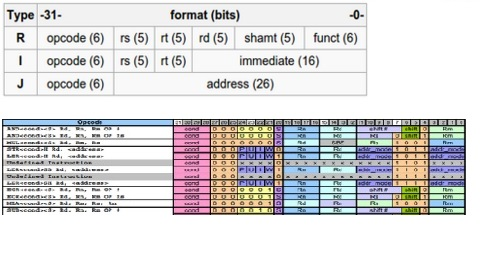
\includegraphics[width=\linewidth]{ARMMIPS.jpg}
  \caption{Instruction format of ARM and MIPS}
  \label{fig:AM}
\end{figure}

 
\item{Atmel AVR based on Harvard architecture, that is, to separate storage and signal pathways for instructions and data. There are several applications base on the AVR architecture, some of famous usage are in Microsoft XBOX controller and vehicle computing system such as in BMW or Daimler Cheysler. }

More RISC-based processors are not list here, but it shows the fact that RISC have been thought as a primary choice for the embedded systems.

\end{itemize}



\section{ARM architecture}

As mentioned at previous section, ARM(Acorn RISC Machine, and changed to Advanced RISC Machines in 1990) architecture is a family of RISC. ARM architecture require fewer transistors than CISC, this approach reduces costs, heat and power use. Compare with most of personal computers processors like intel x86, RISC-based ARM architecture are desirable traits for light, portable, battery powered devices - including smart phones, laptops, tablet and other embedded systems. \cite{ARM1}

\subsection{Introduction}
ARM does not manufacture products, but selling IP (Intellectual Property) cores. This is, ARM only holdings develops the instructions sets and  architecture for ARM-based products. So ARM Holdings licenses the chip designs and the ARM instruction set architectures to third parties, who design their own products which is able to costume their own productions such like system on chip(SoC). Thousands of physical IP users are cooperate with ARM with this strategy.\cite{ARM1}

\begin{figure}[h]
  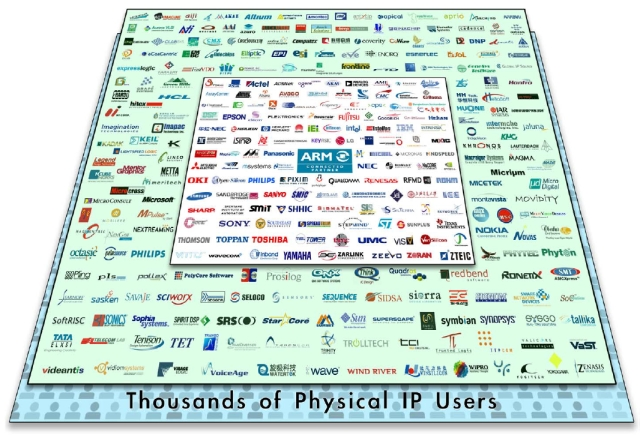
\includegraphics[width=\linewidth]{IPUSER.jpg}
  \caption{Physical IP Users}
  \label{fig:User}
\end{figure}

ARM is one of the most widely used instruction set architecture in terms of quantity produced. Low heat, low cost and low power consumptions make ARM architecture processors popular. According to ARM officially website, " In Q4 of 2013 ARM partners shipped an impressive 2.9 billion ARM-powered chips, taking the full year total to 10 billion chips. ARM has now reached the 50 billion chips milestone", and ARM based chips are used in nearly 60\% of world's mobile devices.\cite{ARM2} Such a astonishing numbers shows the enormous success again. 

\subsection{The first ARM Core}
The first ARM architecture processor ARM1 which based on ARM architecture ARMv1 was released in 1985. The instruction set is similar as 6502 instructions set, because this processor was designed for the BBC's (British Broadcasting Corporation) BBC Micro computer. BBC Micro uses MOS 6502 processor, so ARM1 was following the similar architecture to shorten the development time and technique conversion. Intel 80286 was released in 1982, which designed with 6 to 12 MHz clock speed (2.66 MIPS), 134,000 transistors, 1.5 MIPS chip performance, 1.5 microns circuit size, 16 bits bus width, 16 megabytes addressable memory, 1 gigabyte virtual memory on the 6-inch silicon wafers.\cite{C} Compare with ARM1 which uses 25000 transistors, 6 MHz clock speed, 3 microns circuit size\cite{C}. We can see that ARM1 uses much less transistors, this is also one of the reason that ARM1 require less power and product less heat. October 1985, the same year as ARM1's birth, Intel released the new 80386 chips with 275,000 transistors, and 16MHz clock speed. Henceforward, Intel was thought as highly performance for personal computer's choice, and ARM for the embedded systems. 
\begin{figure}[h]
  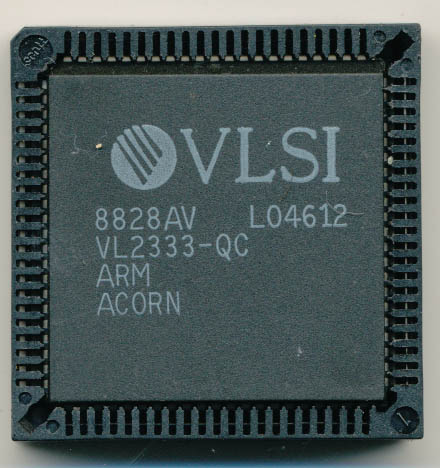
\includegraphics[width=0.7\linewidth]{ARM1.jpg}
  \caption{ARM1 made by VLSI}
  \label{fig:AM}
\end{figure}


\subsection{Important changes of ARM Architecture}
There were several changes for the ARM architecture. Here are the minor changes for the ARM:
\begin{itemize} 
\item{ARMv1} Core Designed: ARM1
\\The first ARM processor architecture. 

\item{ARMv2} Core Designed: ARM2, ARM250, ARM3
\\MUL is added into processor. And the advanced version ARMv2a add Memory control core, Graphic and I/O cores. ARM3 (based on ARMv2a) processor is the first time to build in 4 kb cache.  

\item{ARMv3} Core Designed: ARM6, ARM7
\\Extend the addressing space. Processors before ARM 6 all uses 26 bits memory address bus, and support up to 64 MB memory, but ARM 6 support 32 bit memory address , and up to 4 GB memory. ARM 7 increase the cache to 8 kb, and also increase the clock speed to 40 MHz.

\item{ARMv4T} Core Designed: ARM7TDMI, ARM9TDMI, SecurCore SC100
\\Except originally 32 bits instruction sets, now support Thumb instruction sets. Thumb is the optimized 16 bits instruction set, according to  ARM officially website, the Thumb can reduce about 35\% of code size. The Thumb Decoder will compress Thumb instructions into 32 bits ARM instructions, so it both take the advantages of the speed of instructions load and execution bu 32 bits memory bus.


\item{ARMv5TEJ} Core Designed: ARM7EJ
\\Jazelle DBX arithmetic  circuit added into ARM7EJ processor. This hardware can increase the speed for most of Java byte code, this directly support the Java programming efficiency. Also it extended new instruction which is fine for DSP instruction such like saturated arithmetic, this helps processor to increase the speed for media applications. 

\item{ARMv5TE} Core Designed: ARM9, ARM10E
\\Before ARM 9, all ARM processors and Intel processors are based on von Neumann architecture. Von Neumann architecture. The ARM 9 is the first ARM processor designed with Harvard architecture which physically separate storage and signal pathways for instructions and data. The advantage  of Harvard architecture is that processor can access data and instruction memory at the same time, so the processor can fetch the next instruction while executing the current one. A comparison figure for von Neumann and Harvard architecture is shown in the Figure 4.

\begin{figure}[h]
  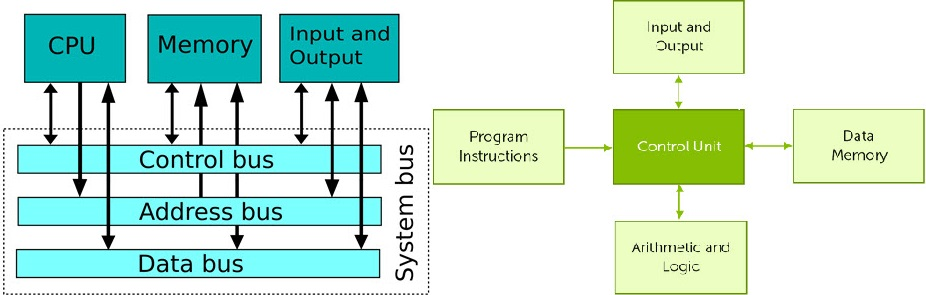
\includegraphics[width=\linewidth]{HV.jpg}
  \caption{Ha vs Von}
  \label{fig:HV}
\end{figure}

\item{ARMv6} Core Designed: ARM11
\\SIMD (Single instruction, multiple data) computing is added. SIMD helps computers with multiple processing elements that perform the same operation on multiple data points simultaneously. This increase the ability to handle multimedias such as digital image and digital audio. And ARMv6 also upgrade Thumb instruction set to Thumb-2, this extend part of 16 bits instructions to 32-bits. One of the most successful production with ARM11 is the Apple iPhone. Figure 5 shows how SIMD works.
\begin{figure}[]
  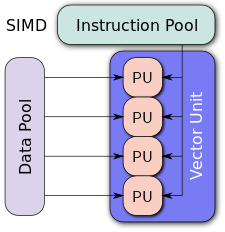
\includegraphics[width=0.3\linewidth]{SIMD.jpg}
  \caption{SIMD}
  \label{fig:SIMD}
\end{figure}


\end{itemize} 



\section{Conclusion}
As this study research shows, the personal embedded system devices become part of contemporary portable equipment. As the manufacturing technique involved on wafers, low heat, low cost and fast microprocessor makes the integrated  circuits gets into another generation. At the end of 2015, wearable electronics becoming a hot topic for the market, Fitbit, smart watches, VR gaming and many others shows that the microprocessor still get a lot potential to be developed.  

%\section{Conclusion}
%The conclusion goes here.




% conference papers do not normally have an appendix


% use section* for acknowledgment
%\section*{Acknowledgment}


%The authors would like to thank...





% trigger a \newpage just before the given reference
% number - used to balance the columns on the last page
% adjust value as needed - may need to be readjusted if
% the document is modified later
%\IEEEtriggeratref{8}
% The "triggered" command can be changed if desired:
%\IEEEtriggercmd{\enlargethispage{-5in}}

% references section

% can use a bibliography generated by BibTeX as a .bbl file
% BibTeX documentation can be easily obtained at:
% http://www.ctan.org/tex-archive/biblio/bibtex/contrib/doc/
% The IEEEtran BibTeX style support page is at:
% http://www.michaelshell.org/tex/ieeetran/bibtex/
%\bibliographystyle{IEEEtran}
% argument is your BibTeX string definitions and bibliography database(s)
%\bibliography{IEEEabrv,../bib/paper}
%
% <OR> manually copy in the resultant .bbl file
% set second argument of \begin to the number of references
% (used to reserve space for the reference number labels box)
\begin{thebibliography}{1}

\bibitem{Textbook}
John L. H., \& David A. P. (2013). "Computer Architecture: A Quantitative Approach Fifth Edition."

\bibitem{A}
Wayne Wolf; Ahmed Amine Jerraya, and Grant Martin, "Multiprocessor System-on-Chip
(MPSoC) Technology," IEEE TRANSACTIONS ON COMPUTER-AIDED DESIGN OF INTEGRATED CIRCUITS AND SYSTEMS, VOL. 27, NO. 10, OCTOBER 2008

\bibitem{B}
What is RSIC. Retrieved from https://cs.stanford.edu/people/eroberts/courses/soco/projects/risc/risccisc/index.html

\bibitem{C}
80286 Microprocessor Package. Retrieved from http://content.cdlib.org/ark:/13030/kt7h4nc9c2/?layout=metadata

\bibitem{D}
ARM Processor, RISC and DISC. Retrieved http://www.techbang.com/posts/10678-fully-understand-arm-processors-cisc-and-risc-are-what-history-structure-a-see-through-the-computer-96-issues-cover-story-the-king?page=1

\bibitem{ARM1}
Clements, A., "ARMs for the poor: Selecting a processor for teaching computer architecture," in Frontiers in Education Conference (FIE), 2010 IEEE , vol., no., pp.T3E-1-T3E-6, 27-30 Oct. 2010

\bibitem{ARM2}
Jaggar, D., "Arm Architecture And Systems," in Micro, IEEE , vol.17, no.4, pp.9-11, July-Aug. 1997

\bibitem{ARM3}
Blem, E.; Menon, J.; Sankaralingam, K., "Power struggles: Revisiting the RISC vs. CISC debate on contemporary ARM and x86 architectures," in High Performance Computer Architecture (HPCA2013), 2013 IEEE 19th International Symposium on , vol., no., pp.1-12, 23-27 Feb. 2013

\end{thebibliography}




% that's all folks
\end{document}


